\documentclass[aspectratio=169]{beamer}

% Je kan het lettertype iets vergroten door hierboven optie ``14pt'' toe te
% voegen.

%==============================================================================
% Aanloop
%==============================================================================

%---------- Vormgeving --------------------------------------------------------

\usetheme{hogent}

% Kies hieronder een achtergrondkleur
\usecolortheme{hgwhite} % witte achtergrond, zwarte tekst
%\usecolortheme{hgblack} % zwarte achtergrond, witte tekst

%---------- Packages ----------------------------------------------------------

\usepackage[dutch]{babel}      % Nederlandse taal: splitsingen, enz.

\usepackage{booktabs}          % Mooie tabellen
\usepackage{multirow,multicol} % Tabelcellen samenvoegen
\usepackage{eurosym}           % Euro symbool
\usepackage{hyperref}
\usepackage{bbding}
\usepackage{tabularx}
\hypersetup{
    colorlinks=true,
    linkcolor=blue,
    filecolor=magenta,      
    urlcolor=cyan,
    pdftitle={Overleaf Example},
    pdfpagemode=FullScreen,
}

\urlstyle{same}

%---------- Commando-definities -----------------------------------------------

%---------- Info over de presentatie ------------------------------------------

\title[Korte titel]{Google Scholar zoekresultaten voor wetenschappelijke projecten: linked data \& natural language processing}
\author{Bart De Paepe}
\date{16 juni 2025}

%==============================================================================
% Inhoud presentatie
%==============================================================================

\begin{document}

%---------- Titelpagina, inhoudstafel -----------------------------------------

\frame{\maketitle}

\begin{frame}
  \frametitle{Inhoud.}

  \tableofcontents
\end{frame}
 
%---------- Corpus ------------------------------------------------------------

\section{Kader.}

\begin{frame}
  \frametitle{Vlaams Instituut voor de Zee}
  \begin{figure}
     
\includegraphics[height=.4\textheight]
      {kader/VLIZ_LOGO.png}
      % Bron: https://www.pexels.com/photo/hand-on-cup-of-coffee-984536/
      
  \end{figure}
  \centering
  \url{https://www.vliz.be}
  
\end{frame}

\begin{frame}
    \frametitle{Integrated Marine Information System}
    \begin{figure}
            
\includegraphics[height=.5\textheight]
            {kader/imis.jpg}
            % Bron: https://www.pexels.com/photo/hand-on-cup-of-coffee-984536/
    \end{figure}
    \centering
    \url{https://www.vliz.be/nl/imis}
    
\end{frame}

\begin{frame}
    \frametitle{Google Scholar}
    \begin{columns}[c]
        % create the column with the first image, that occupies
        % half of the slide
        \begin{column}{.5\textwidth}
            \centering
    \begin{figure}
        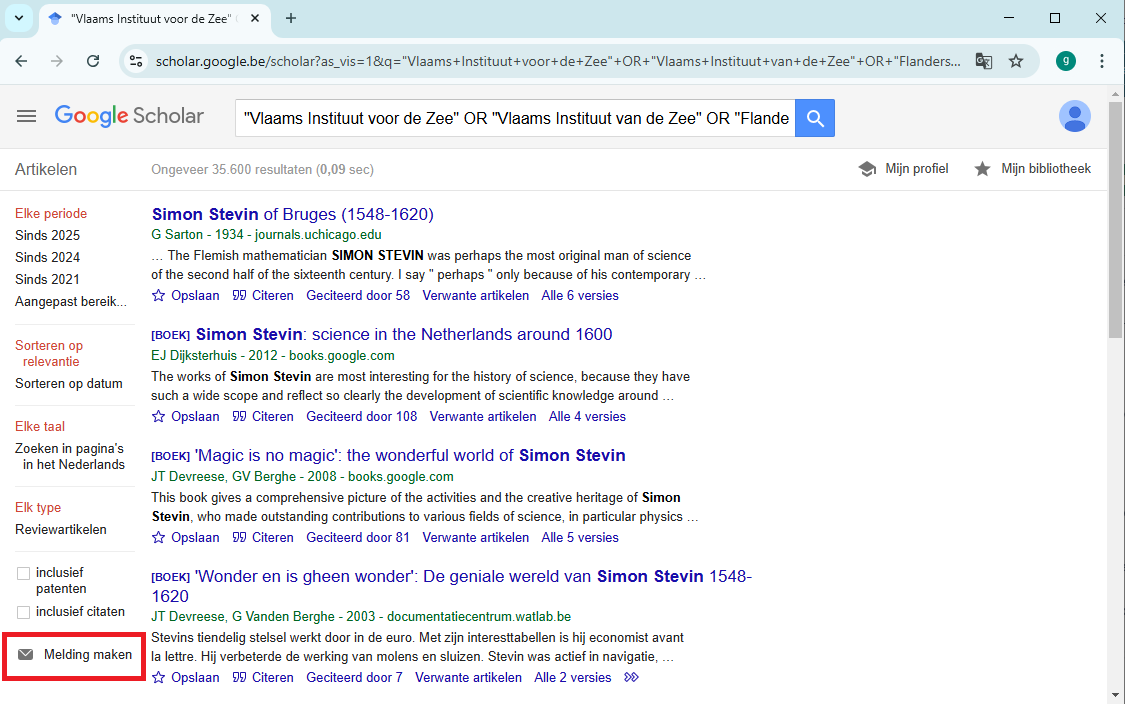
\includegraphics[height=.5\textheight]
        {kader/google-scholar/2_zoekresultaten.PNG}
        % Bron: https://www.pexels.com/photo/hand-on-cup-of-coffee-984536/
        
    \end{figure}
    zoekopdracht
    \end{column}
    \begin{column}{.5\textwidth}
        \centering
    \begin{figure}
        
        
        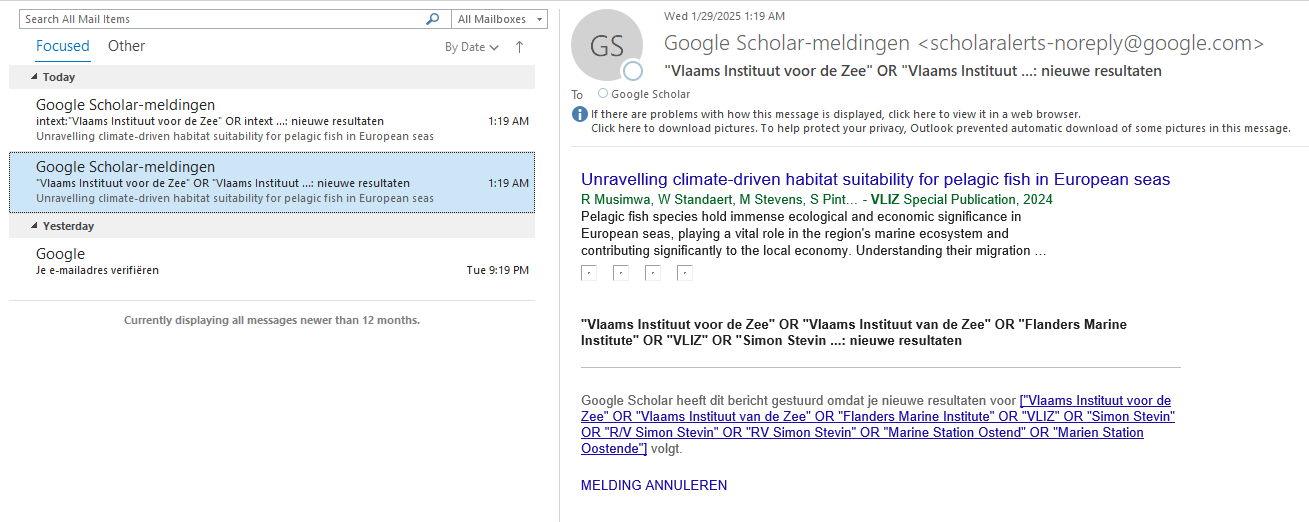
\includegraphics[height=.5\textheight]
        {kader/google-scholar/5_email.PNG}
        % Bron: https://www.pexels.com/photo/hand-on-cup-of-coffee-984536/
        
    \end{figure}
    alert
\end{column}
\end{columns}
    
    
\end{frame}


\begin{frame}
    \frametitle{De onderzoeksvraag.}
    \tiny
    \colorbox{hgorange}{``Hoe kunnen de zoekresultaten van Google Scholar automatisch toegevoegd worden aan IMIS?''}
    \begin{itemize}
        \item Hoe kunnen de uiteenlopende zoekresultaten van Google Scholar omgezet worden in gestructureerde data?
        \item Zijn alle zoekresultaten uniek identificeerbaar zodat er geen duplicaten opgeslagen worden?
    \end{itemize}
    \begin{itemize}
        \item Hoe kunnen ook steeds nieuwe zoekresultaten van dezelfde zoekopdracht systematisch opgezocht worden?
        \item Kan er een score berekend worden hoe relevant elk zoekresultaat is ten opzichte van de zoekopdracht?
        \item Als er geen unieke identifier is, hoe wordt er dan gecontroleerd op duplicaten? 
    \end{itemize}
    \begin{itemize}
        \item Hoe blijft de tool overwegend onafhankelijk van third-party software?
        \item Hoe wordt er gegarandeerd dat de tool op de bestaande hardware kan draaien? 
    \end{itemize}
    
    
\end{frame}

{
    \setbeamertemplate{background}[pure]{methode/arrow.png}
\section{Proof of \linebreak Concept.}
}

\begin{frame}[t]
    \frametitle{Web scraping (1/2).}
    \begin{columns}[t]
        % create the column with the first image, that occupies
        % half of the slide
        \begin{column}{.5\textwidth}
            \begin{figure}
                
                
                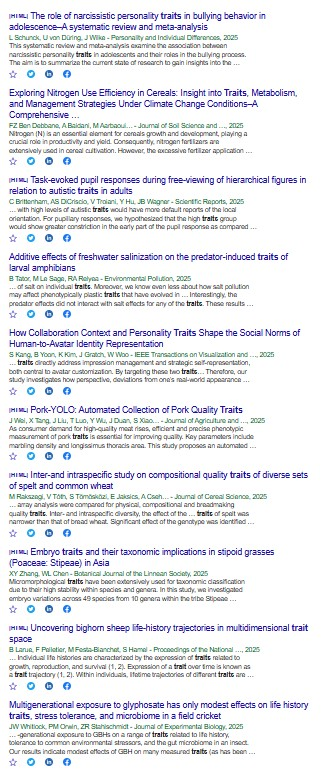
\includegraphics[height=1.5\textheight]
                {methode/web-scraping/SERP.jpg}
                % Bron: https://www.pexels.com/photo/hand-on-cup-of-coffee-984536/
                
            \end{figure}
            
        \end{column}
        \begin{column}{.5\textwidth}
            
            \begin{listing}
                
                    \tiny
                    \textbf{parse with LLM}\\
                    messages=[
                    {"role": "system",
                        "content": "You are a master at scraping Google Scholar results data. Scrape top 10 organic results data from Google Scholar search result page."},
                    ],
                
                
            \end{listing}
            \vspace{.3cm}
            \hrule
            \vspace{.3cm}
            \begin{listing}
                
                    \tiny
                    \textbf{parse with scraper}\\
                    <h3 style="font-weight:normal;margin:0;font-size:17px;line-height:20px;">
                    <span style="fon...lign:2px">[HTML]</span>    
                    <a href="https://www.s...8" \colorbox{hgorange}{class="gse\_alrt\_title"} style="f...t:22px">
                    The role of narcissistic personality <b>traits </b>in bullying behavior 
                    in adolescence–A systematic review and meta-analysis
                    </a>
                    </h3>
                    <div \colorbox{hgorange}{class="gse\_alrt\_sni"} style=3D"line-height:17px">The Ocean Race, known as one of the world most challenging round-the-world <br>
                    sailing competitions, has evolved into a significant platform for ocean science, <br>
                    advocacy, and innovation. Through its Science Program, The Race leverages its...</div>
                
                
            \end{listing}
        \end{column}
    \end{columns}
\end{frame}

\begin{frame}
    \frametitle{Web scraping (2/2).}
    \begin{columns}[c]
        % create the column with the first image, that occupies
        % half of the slide
        \begin{column}{.5\textwidth}
    \begin{itemize}
        \item \XSolidBrush OpenAI (AKA ChatGPT)
        \item \XSolidBrush Anthropic (met Mirascope)
        \item \XSolidBrush Llama 3 (met Ollama)
        \item \XSolidBrush Serpapi
        \item \Checkmark Beautiful Soup
    \end{itemize}
\end{column}
\begin{column}{.5\textwidth}
    \begin{figure}
        
        
        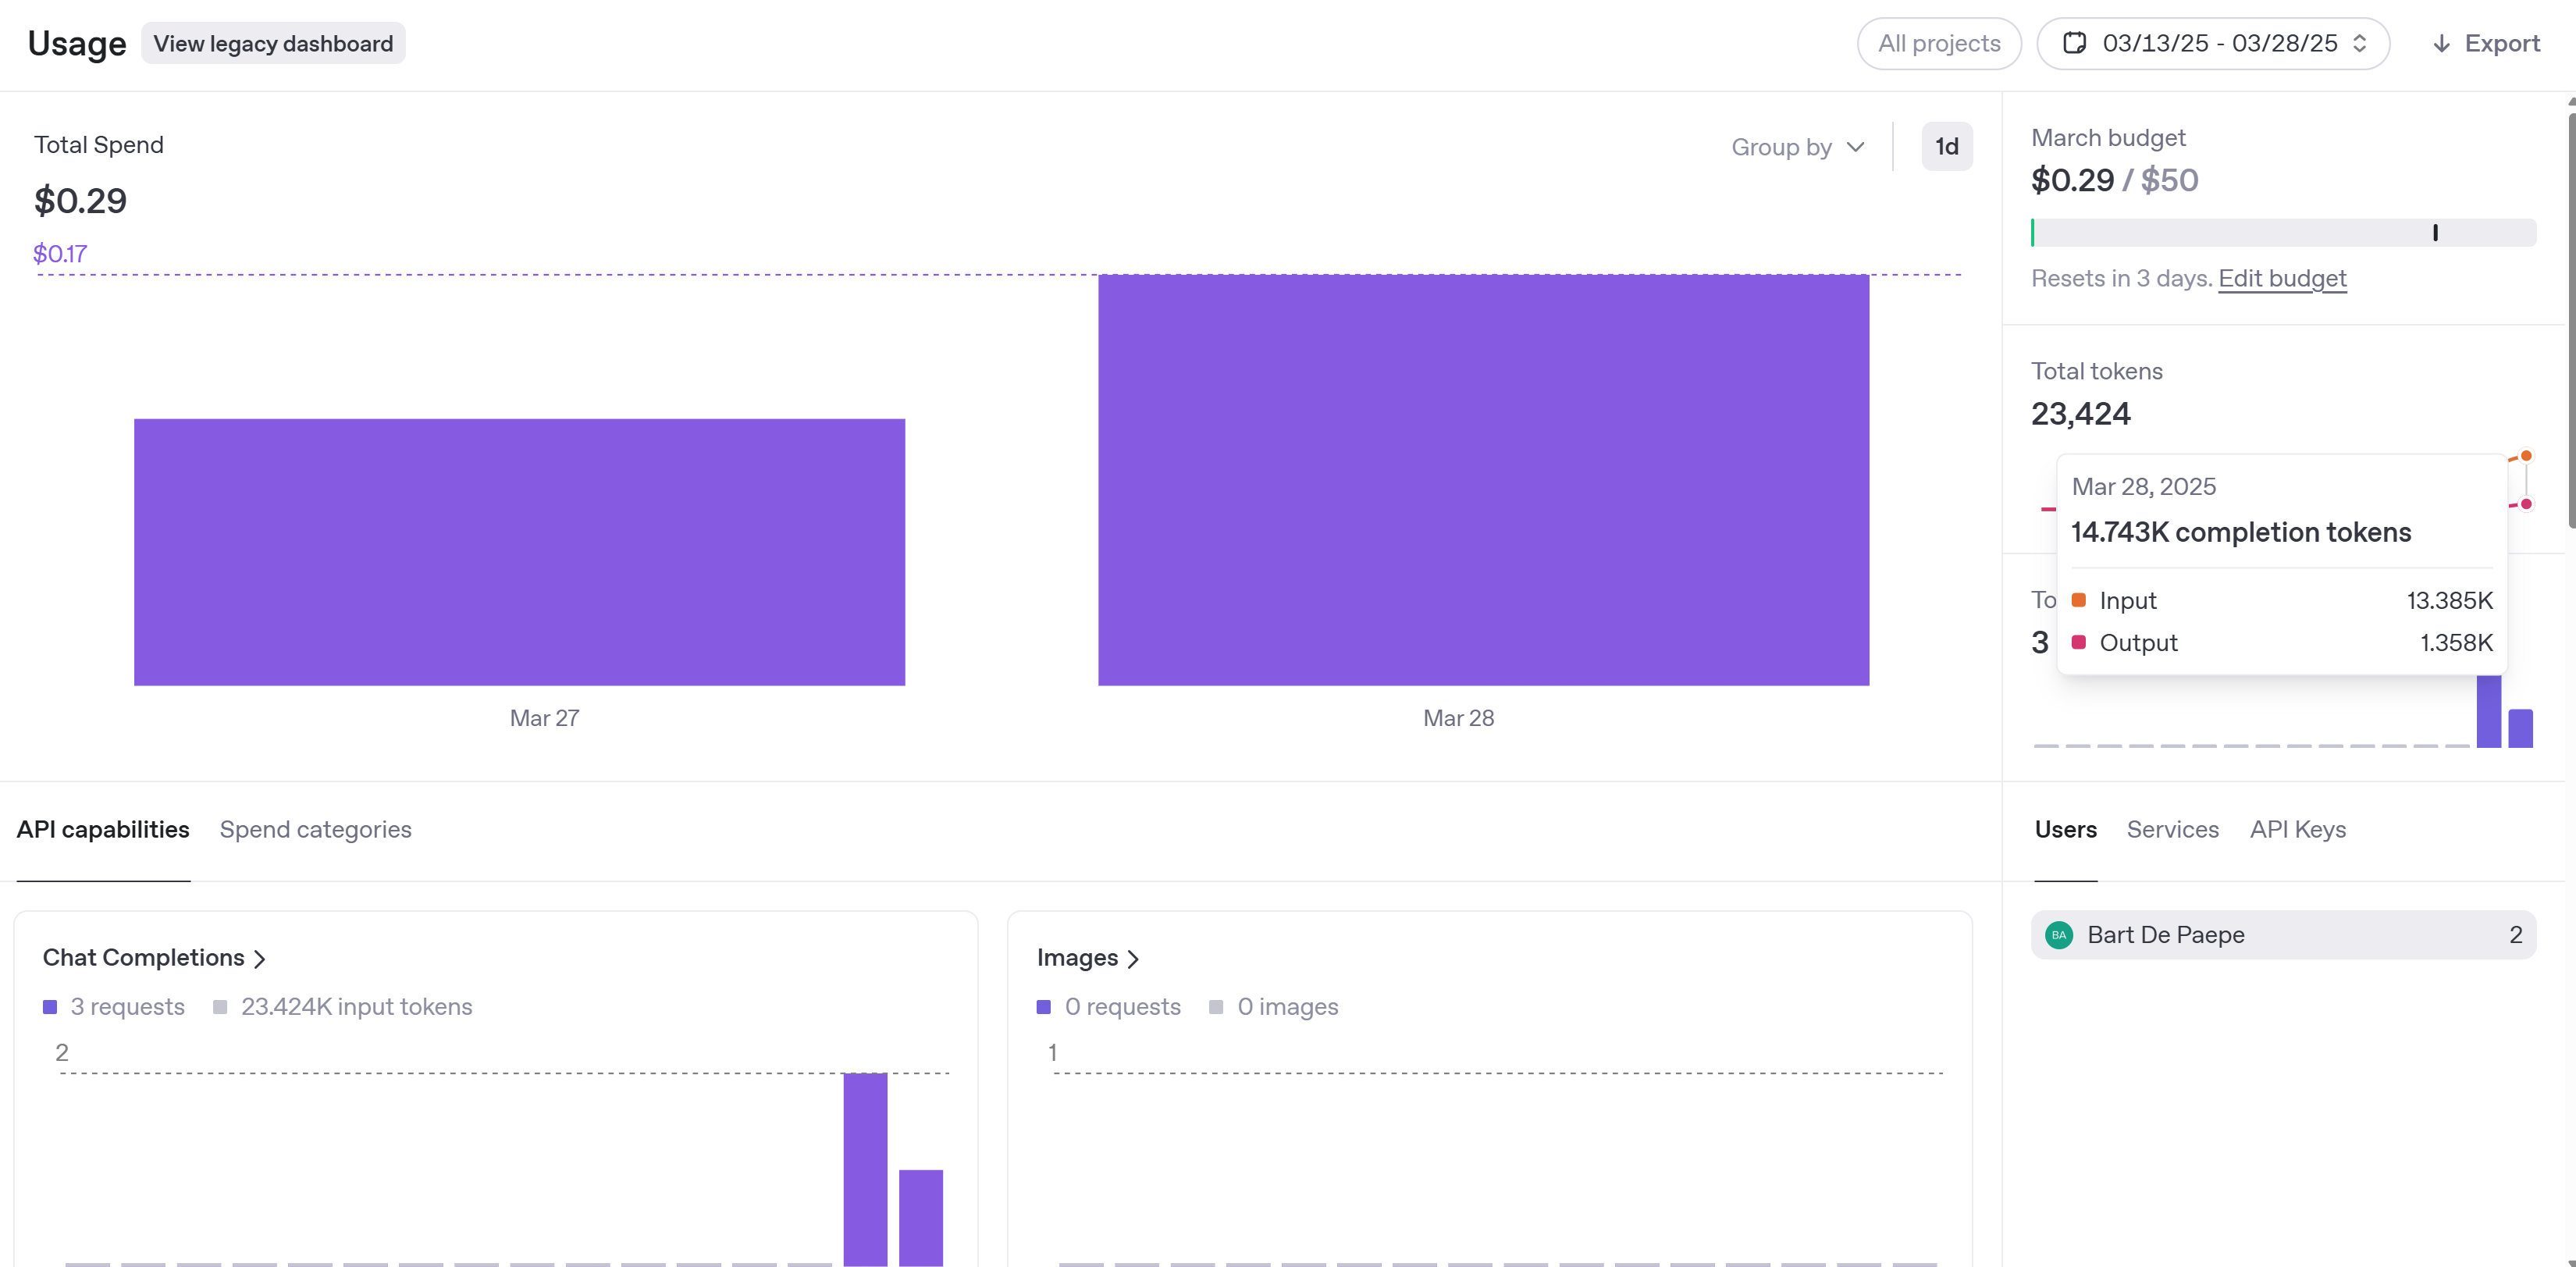
\includegraphics[height=.5\textheight]
        {methode/web-scraping/openai_billing.png}
        % Bron: https://www.pexels.com/photo/hand-on-cup-of-coffee-984536/
        
    \end{figure}
\end{column}
\end{columns}
\end{frame}

\begin{frame}
\frametitle{Natural language processing.}
\begin{itemize}
    \item ``Het \colorbox{hgorange}{VLIZ} verwelkomt nieuwsgierige particulieren en kleine groepen voor een bezoek aan haar Campus en haar Mariene Station Oostende.''
    \item \begin{enumerate}
        \item Coreference resolution
        \item Stopwoorden
        \item Lemmatisering
    \end{enumerate}
    \item ``\colorbox{hgorange}{VLIZ} verwelkom nieuwsgierig particulier klein groep bezoek \colorbox{hgorange}{VLIZ} Campus \colorbox{hgorange}{VLIZ} Marien Station Oostende.''
\end{itemize}
\[
relevantiescore = frequentie \ast log\left(\frac{totaal \hspace{1mm} aantal \hspace{1mm}  zoekresultaten}{aantal \hspace{1mm}  zoekresultaten \hspace{1mm}  waar \hspace{1mm}  term \hspace{1mm}  voorkomt}\right)
\] 



\end{frame}

\begin{frame}
\frametitle{Linked data.}
\begin{columns}[c]
    % create the column with the first image, that occupies
    % half of the slide
    \begin{column}{.5\textwidth}
        \centering
        \[https://pubs.acs.org/doi/full/10.1021/acsami.4c21991\]
        \begin{figure}
            
            
            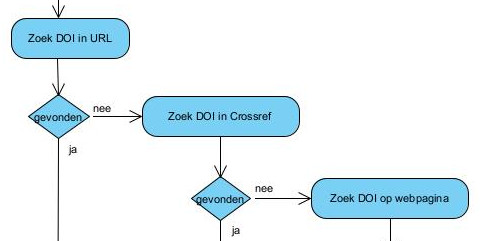
\includegraphics[height=.5\textheight]
            {methode/linked-data/DOI_flow.jpg}
            % Bron: https://www.pexels.com/photo/hand-on-cup-of-coffee-984536/
            
        \end{figure}
    \end{column}
    \begin{column}{.5\textwidth}
        \centering
        verschillende types webpagina's
        \begin{itemize}
            \item een gewone HTML pagina
            \item een PDF document
            \item een webpagina met een embedded PDF document
        \end{itemize}
    \end{column}
\end{columns}
\end{frame}

\begin{frame}
\frametitle{Semantic search.}

    \begin{columns}[c]
        % create the column with the first image, that occupies
        % half of the slide
        \begin{column}{.7\textwidth}
            \centering
            \begin{figure}
                
                
                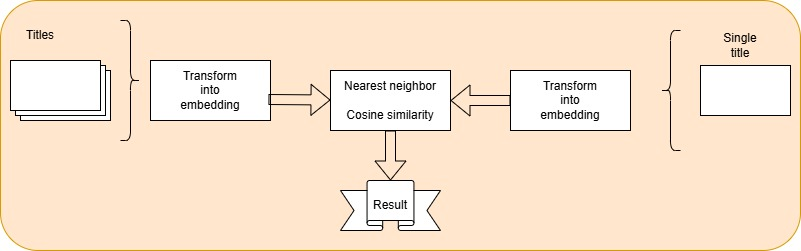
\includegraphics[height=.38\textheight]
                {methode/semantic-search/embeddings.jpg}
                % Bron: https://www.pexels.com/photo/hand-on-cup-of-coffee-984536/
                
            \end{figure}
            
            
            
        \end{column}
        \begin{column}{.3\textwidth}
            \centering
            \begin{figure}
                
                
                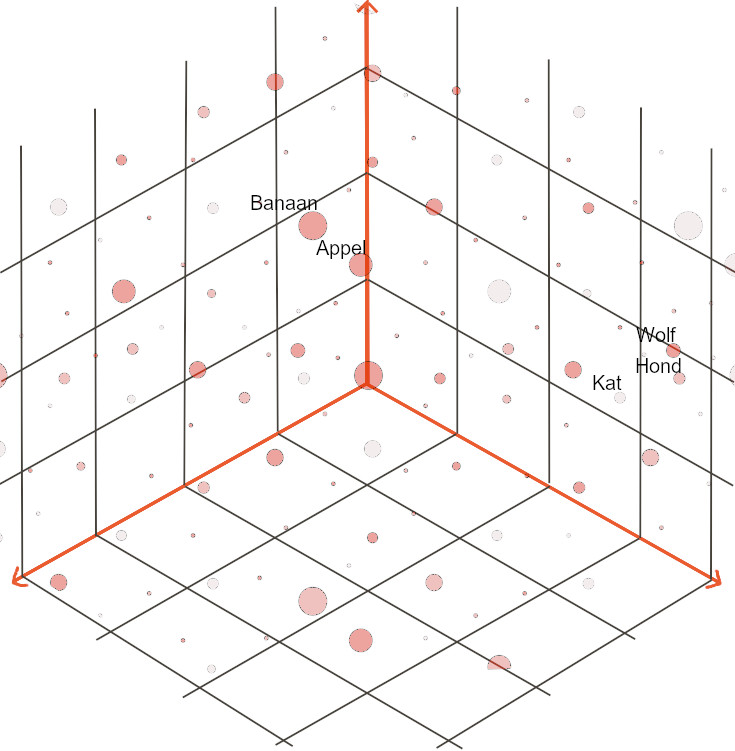
\includegraphics[height=.5\textheight]
                {methode/semantic-search/word2vec2.jpg}
                % Bron: https://www.pexels.com/photo/hand-on-cup-of-coffee-984536/
                
            \end{figure}
        \end{column}
    \end{columns}
    
    


\end{frame}



\section{Resultaten.}


\begin{frame}
    \frametitle{Resultaten (1/4).}
    \begin{columns}[c]
        % create the column with the first image, that occupies
        % half of the slide
        
        \begin{column}{.5\textwidth}
            \centering
            \begin{figure}
                
                
                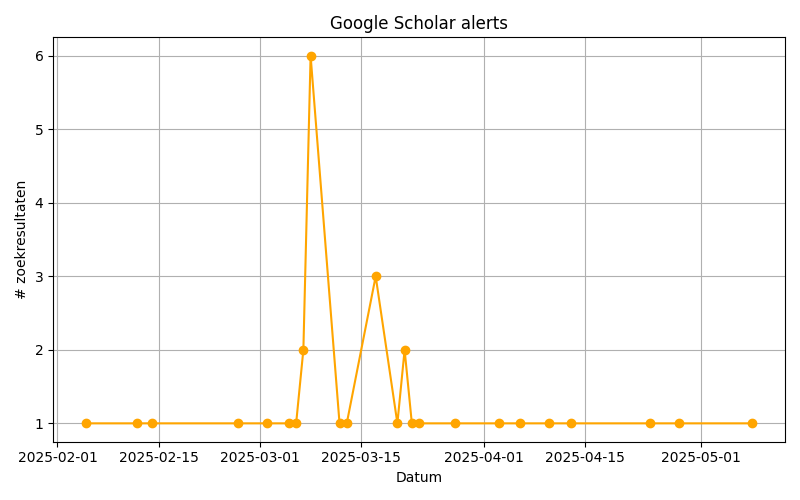
\includegraphics[height=.5\textheight]
                {resultaten/GS_alerts_timeline.png}
                % Bron: https://www.pexels.com/photo/hand-on-cup-of-coffee-984536/
                
            \end{figure}
            Zoekresultaten voor de zoekopdracht ``VLIZ''
        \end{column}
        \begin{column}{.5\textwidth}
            \begin{itemize}
                \item 23 alerts
                \item 1-6 zoekresultaten per alert
                \item 18\% van de zoekresultaten zijn volledig
            \end{itemize}
            \begin{figure}
                
                
                
\includegraphics[height=.2\textheight]
                {resultaten/GS_alerts_auteurtijdschriftjaartal.jpg}
                % Bron: https://www.pexels.com/photo/hand-on-cup-of-coffee-984536/
                
            \end{figure}
        \end{column}
    \end{columns}
    
\end{frame}

\begin{frame}
\frametitle{Resultaten (2/4).}


\begin{figure}
    
    
    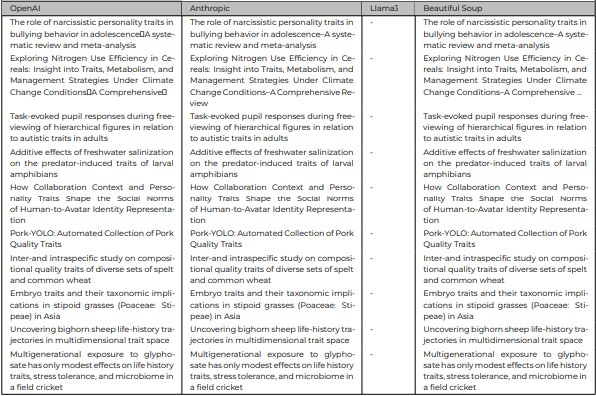
\includegraphics[height=.8\textheight]
    {resultaten/vergelijking_scraping.jpg}
    % Bron: https://www.pexels.com/photo/hand-on-cup-of-coffee-984536/
    
\end{figure}




\end{frame}

\begin{frame}
\frametitle{Resultaten (3/4).}
\begin{columns}[c]
    % create the column with the first image, that occupies
    % half of the slide
    \begin{column}{.5\textwidth}
        \centering
        relevantiescore
        \begin{figure}
            
            
            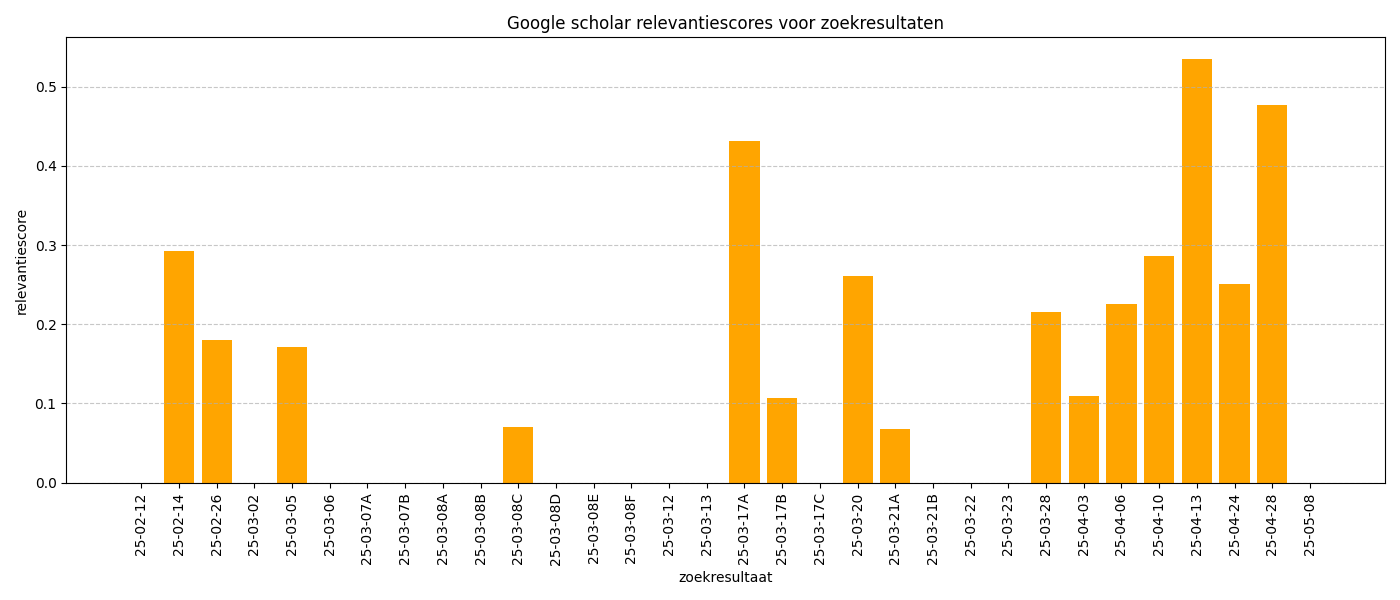
\includegraphics[height=.3\textheight]
            {resultaten/GS_alerts_relevantiescore.png}
            % Bron: https://www.pexels.com/photo/hand-on-cup-of-coffee-984536/
            
        \end{figure}
    \end{column}
    \begin{column}{.5\textwidth}
        \centering
        DOI
            \begin{table}
                \tiny
                \begin{tabular}{ll{3cm}}
                    \toprule
                    & VLIZ & IMIS \\
                    & dataset & dataset \\
                    \midrule
                    Percentage aantal keer dat de  & 48\% & 62,7\% \\
                    DOI gevonden is. &  & \\
                    \midrule
                    \CircleSolid Percentage aantal keer dat  &7\% & \\
                    de DOI in de URL staat. & & \\
                    \CircleSolid Percentage aantal keer dat &20\% & \\
                    de DOI via Crossref gevonden wordt. & \\
                    \CircleSolid Percentage aantal keer dat &73\% & \\
                     de DOI op webpagina staat. & \\
                     \midrule
                     Referentiepercentage DOI & & 61\% \\
                    \bottomrule
                \end{tabular}
                
                
            \end{table}
            
        
    \end{column}
\end{columns}

\end{frame}

\begin{frame}
    \frametitle{Resultaten (4/4).}
    \begin{columns}[c]
        % create the column with the first image, that occupies
        % half of the slide
        
        \begin{column}{.5\textwidth}
            \centering
            semantic search score
            \begin{figure}
                
                
                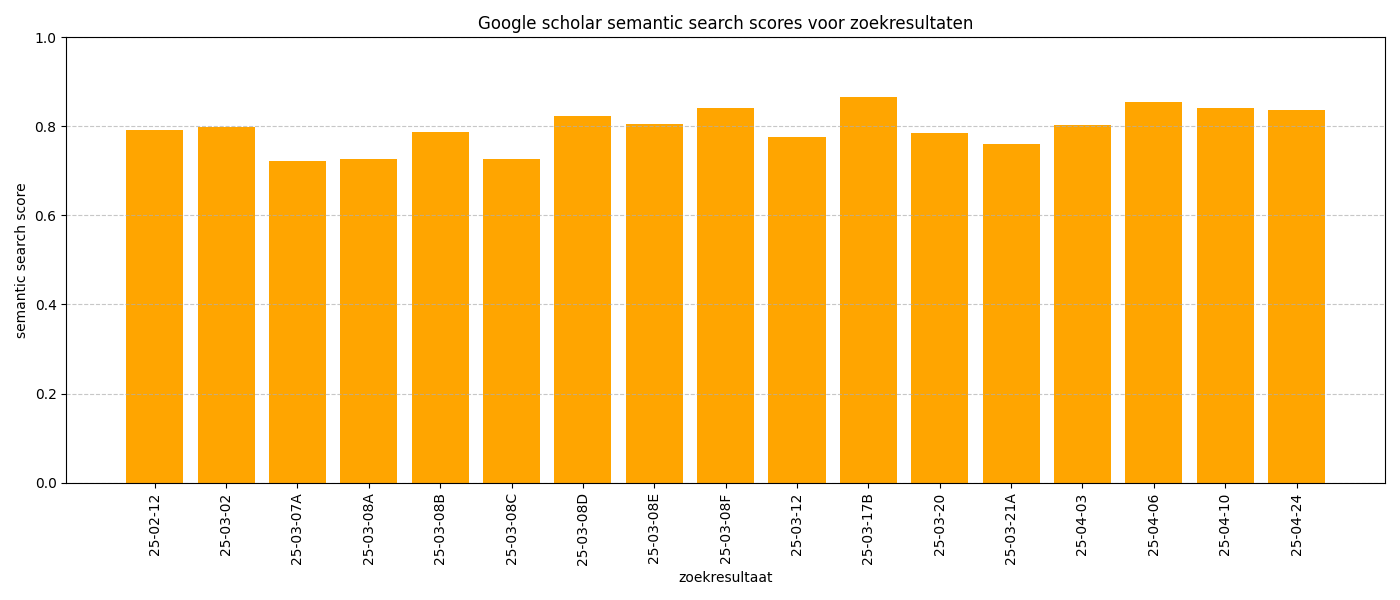
\includegraphics[height=.3\textheight]
                {resultaten/GS_alerts_semanticsearchscore.png}
                % Bron: https://www.pexels.com/photo/hand-on-cup-of-coffee-984536/
                
            \end{figure}
            
        \end{column}
        \begin{column}{.5\textwidth}
            \begin{table}
                \tiny
                \begin{tabularx}{\textwidth}{|X|p{1cm}|} 
                    \hline
                    \textbf{Titel}&\textbf{Semantic search score}\\
                    \hline
                    Genome-wide association study revealed candidate genes associated with egg-laying time traits in layer chicken&\textcolor{orange}{1.0}\\
                    \hline
                    Genome wide association study revealed candidate genes associated with egg laying time traits in layer chicken&\textcolor{orange}{0.99581}\\
                    \hline
                    Gen. wide assoc. study revealed candidate genes associated with egg time traits in layer chicken&\textcolor{orange}{0.970841}\\
                    \hline
                    Genome-wide association study revealed candidate genes associated with egg-laying time traits&\textcolor{orange}{0.954331}\\
                    \hline
                    ... & \textcolor{orange}{\textbf{0.9}}\\
                    \hline
                    Genome-wide association study revealed some new candidate genes associated with flowering and maturity time of soybean in Central and West Siberian regions of Russia&0.81463\\
                    \hline
                    Genome- and Exome-Wide Association Studies Revealed Candidate Genes Associated with DaTscan Imaging Features&0.79323\\
                    \hline
                    ... &  ... \\
                    \hline
                \end{tabularx}
                
                
            \end{table}
        \end{column}
    \end{columns}
    
\end{frame}

\section{Discussie.}

\begin{frame}
\frametitle{Discussie.}
\begin{itemize}
    \item Het automatisch opzoeken van de DOI is de grootste meerwaarde van de tool.
    \item Gebruikers kunnen focussen op publicaties zonder DOI en/of met een lage relevantiescore.
    \item 1500-2000 publicaties per jaar: 5-6 maanden
    \item Met de tool potentiële verlaging tot 2-3 maanden
    \end{itemize}


\end{frame}

\section{Conclusie.}

\begin{frame}
\frametitle{Conclusie.}
\begin{itemize}
    \item De tool zal gebruikt worden binnen het VLIZ.
    \item Korte termijn: Verbetering van de tool door meer gelinkte data (auteurs, tijdschriften) op te zoeken in IMIS.
    \item Lange termijn: Uitvoerige tests met LLMs (zijn niet onderhevig aan de structuur van de HTML)
\end{itemize}

\end{frame}

\begin{frame}
    \frametitle{Woord van dank.}
    \begin{itemize}
        \item Bart Vanhoorne
        \item Milan Lamote
        \item Jan Claes
        \item Fons Verheyde
        \item Cedric Decruw
        \item Lies Knockaert
    \end{itemize}
    
\end{frame}

% Extra slides



\begin{frame}
    \frametitle{Linked data (1).}
    \begin{columns}[c]
        % create the column with the first image, that occupies
        % half of the slide
        \begin{column}{.5\textwidth}
            \centering
            \begin{figure}
                
                
                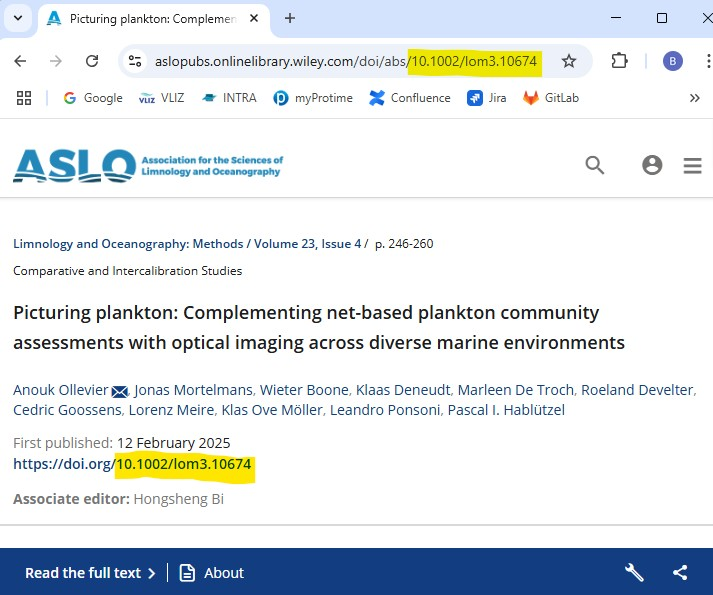
\includegraphics[height=.5\textheight]
                {methode/linked-data/DOI_Link.jpg}
                % Bron: https://www.pexels.com/photo/hand-on-cup-of-coffee-984536/
                
            \end{figure}
            DOI in de URL \& op de webpagina
            
        \end{column}
        \begin{column}{.5\textwidth}
            \centering
            \begin{figure}
                
                
                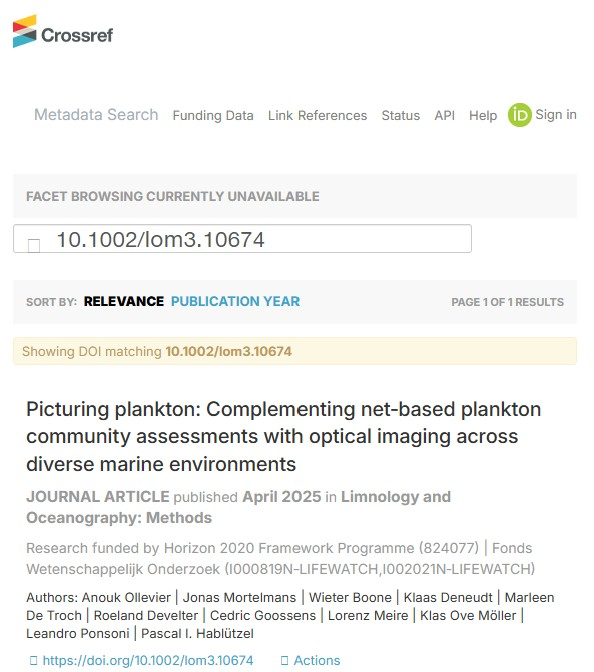
\includegraphics[height=.5\textheight]
                {methode/linked-data/DOI_Crossref.jpg}
                % Bron: https://www.pexels.com/photo/hand-on-cup-of-coffee-984536/
                
            \end{figure}
            DOI in Crossref
        \end{column}
    \end{columns}
\end{frame}

\begin{frame}
    \frametitle{Semantic search (2).}
    \begin{columns}[c]
        % create the column with the first image, that occupies
        % half of the slide
        \begin{column}{.3\textwidth}
            \centering
            \begin{figure}
                
                
                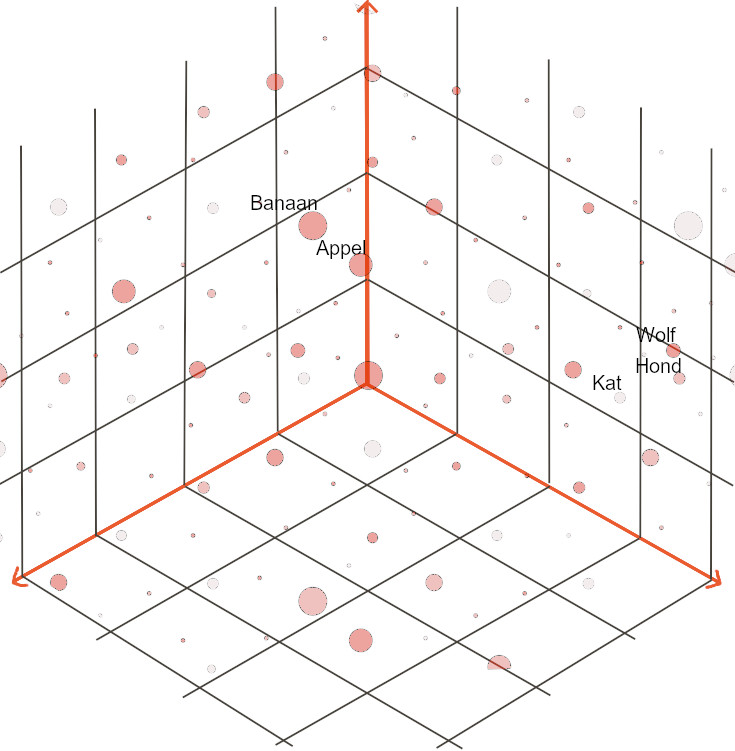
\includegraphics[height=.5\textheight]
                {methode/semantic-search/word2vec2.jpg}
                % Bron: https://www.pexels.com/photo/hand-on-cup-of-coffee-984536/
                
            \end{figure}
            embeddings
        \end{column}
        \begin{column}{.8\textwidth}
            \centering
            \begin{figure}
                
                
                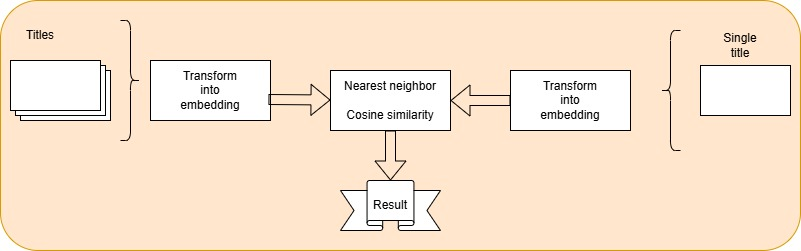
\includegraphics[height=.4\textheight]
                {methode/semantic-search/embeddings.jpg}
                % Bron: https://www.pexels.com/photo/hand-on-cup-of-coffee-984536/
                
            \end{figure}
            schema
        \end{column}
    \end{columns}
\end{frame}


\begin{frame}
    \frametitle{Proof of Concept}
    \begin{figure}
        
        
        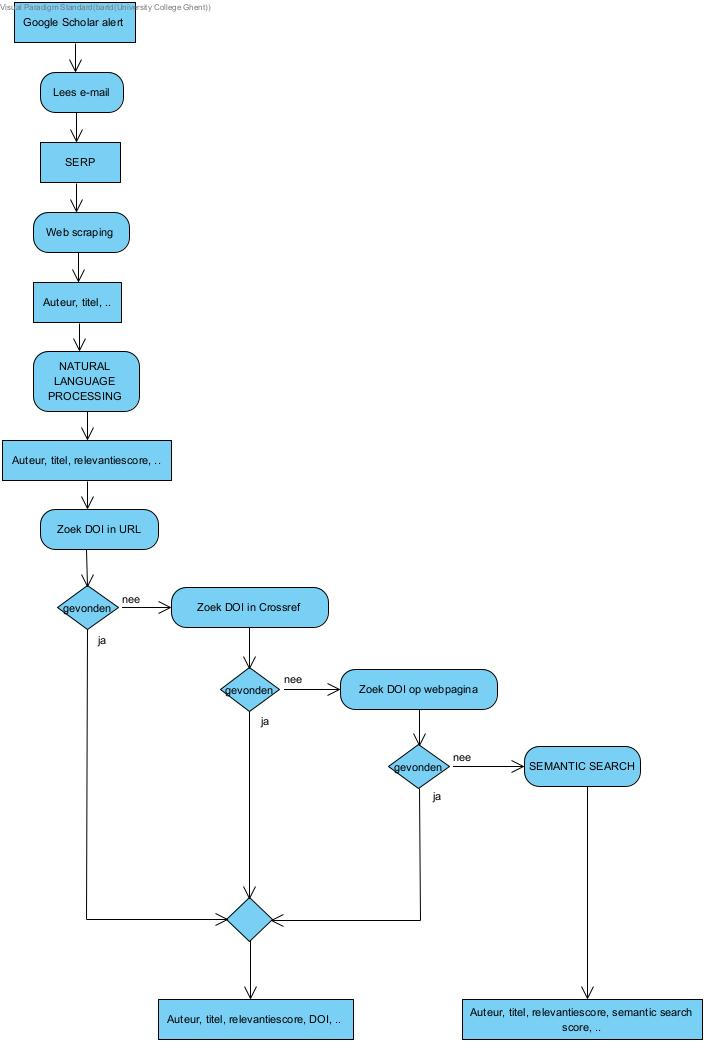
\includegraphics[width=0.35\textwidth]
        {methode/activity-diagram.jpg}
        % Bron: https://www.pexels.com/photo/hand-on-cup-of-coffee-984536/
        
    \end{figure}
    
\end{frame}


\end{document}
